\subsection{Task 3 Results}
\label{sec:task3results}

As described in \ref{sec:task3}, the geometric dimensions are set for the optimized case of Re = 724 including the optimized L segment length. The sample geometry for such geometry is found on Figure \ref{fig:task3sketch}

\begin{figure}[H]
    \centering
    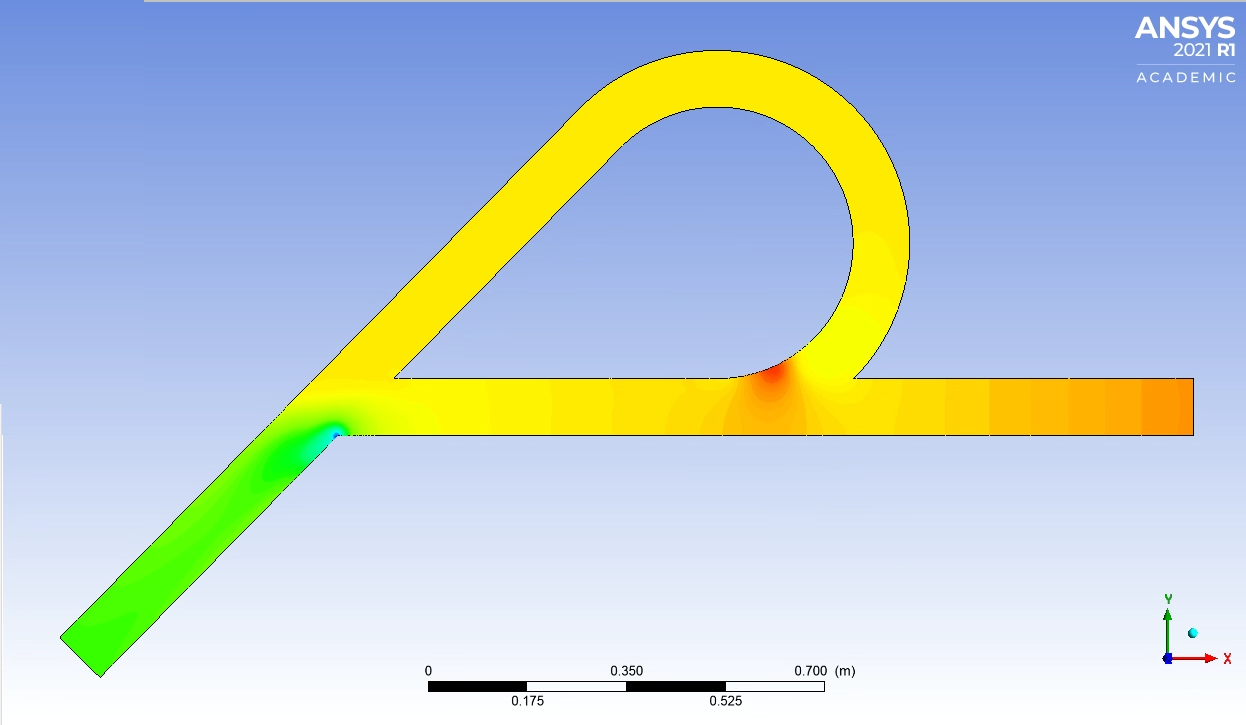
\includegraphics[width=.7\textwidth]{images/task3/sketch.png}
    \caption{Geometry for Task 3}
    \label{fig:task3sketch}
\end{figure}

A mesh size of $5x10^{-3}$ with 300.000+ elements and nodes since ANSYS Student version cannot handle any finer mesh than that value for this case. The necessary plots are given on Figure \ref{fig:omega_epsilon}. It should be noted that while the $k - \omega$ solver struggled highly with the calculations, needing more than 3 times the iterations that $k- \epsilon$ needed. Also, when a reversed flow on a face has occurred, it was seen that the $k - \omega$ solver started to struggle especially, failing to converge properly. \\

When the two models are compared, it can be clearly seen that $k - \omega$ solver has computed more intuitive values especially near the walls as excepted. Since it does not need damping functions like its alternative, it does not inherit their drawbacks, causing in less inaccuracy. The $k - \omega$ solver has shown greater values of pressure near the walls and the areas where this low pressures occur are more continuous and show a more gradient fashion instead of sharply cut sections like $k - \epsilon$ shows. It is likely due to this reason that for most of the geometry, the $k - \epsilon$ solver has calculated higher values of velocity around the valvular conduit whereas its alternative resulted in slightly lower magnitudes of velocity. However, their calculated diodicities are highly in agreement. Table \ref{} shows their resulting diodicity values.\\

\begin{table}[H]
\centering
\caption{Comparison of Diodicities}
\label{tab:compared_diodicities}
\resizebox{.4\textwidth}{!}{%
\begin{tabular}{l|ll}
Solver Type & $k - \omega$ & $k - \epsilon$ \\ \hline
Diodicity   & 2.66         & 2.60          
\end{tabular}%
}
\end{table}

As expected, these values are higher than any other diodicity calculated for this project since we have optimized many dimensions accordingly. Also, the turbulent behavior of flow in this configuration helps with more aggressive drops and changes throughout the valve.

\begin{figure}[H]
 \centering
\begin{subfigure}{.45\textwidth}
  \centering
  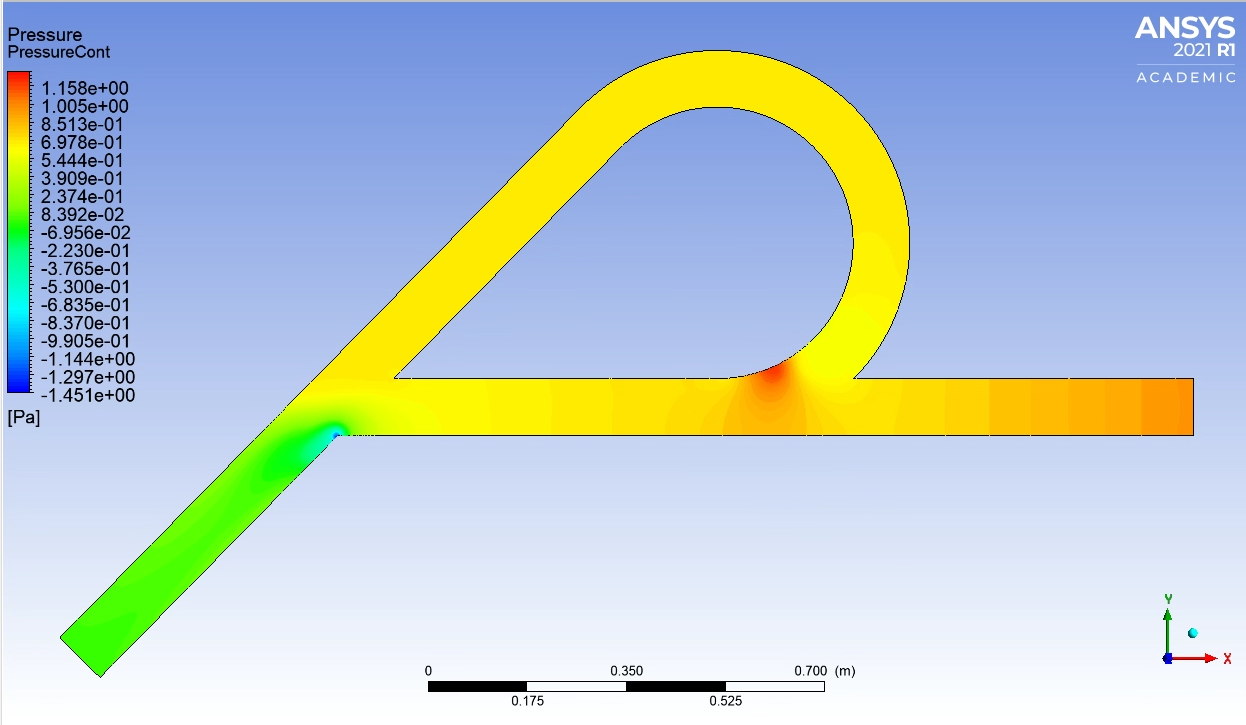
\includegraphics[width=.94\linewidth]{images/task3/epsilon_forward_pressure.png}
  \caption{$k-\epsilon$ Forward Flow Pressure Contours}
  \label{fig:x_d_norm}
\end{subfigure}%
~
\begin{subfigure}{.45\textwidth}
  \centering
  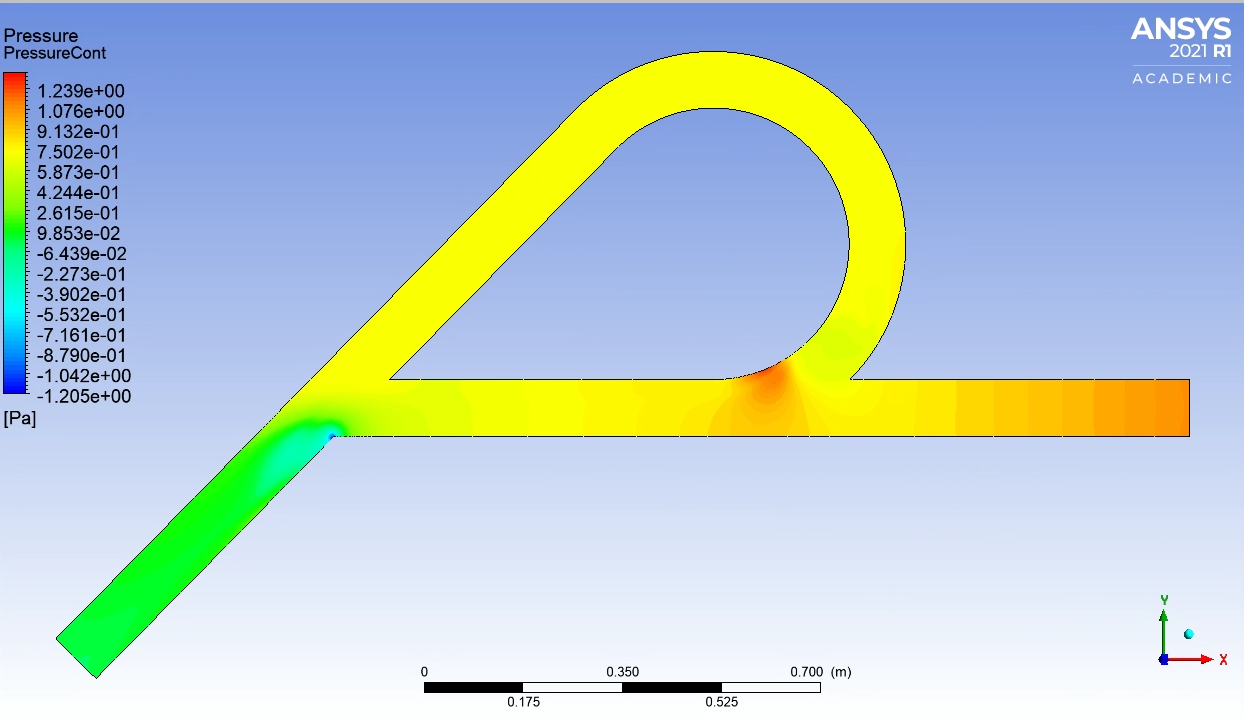
\includegraphics[width=.94\linewidth]{images/task3/omega_forward_pressure.png}
  \caption{$k-\omega$ Forward Flow Pressure Contours}
  \label{fig:x_d_norm_actual}
\end{subfigure}
~
\begin{subfigure}{.45\textwidth}
  \centering
  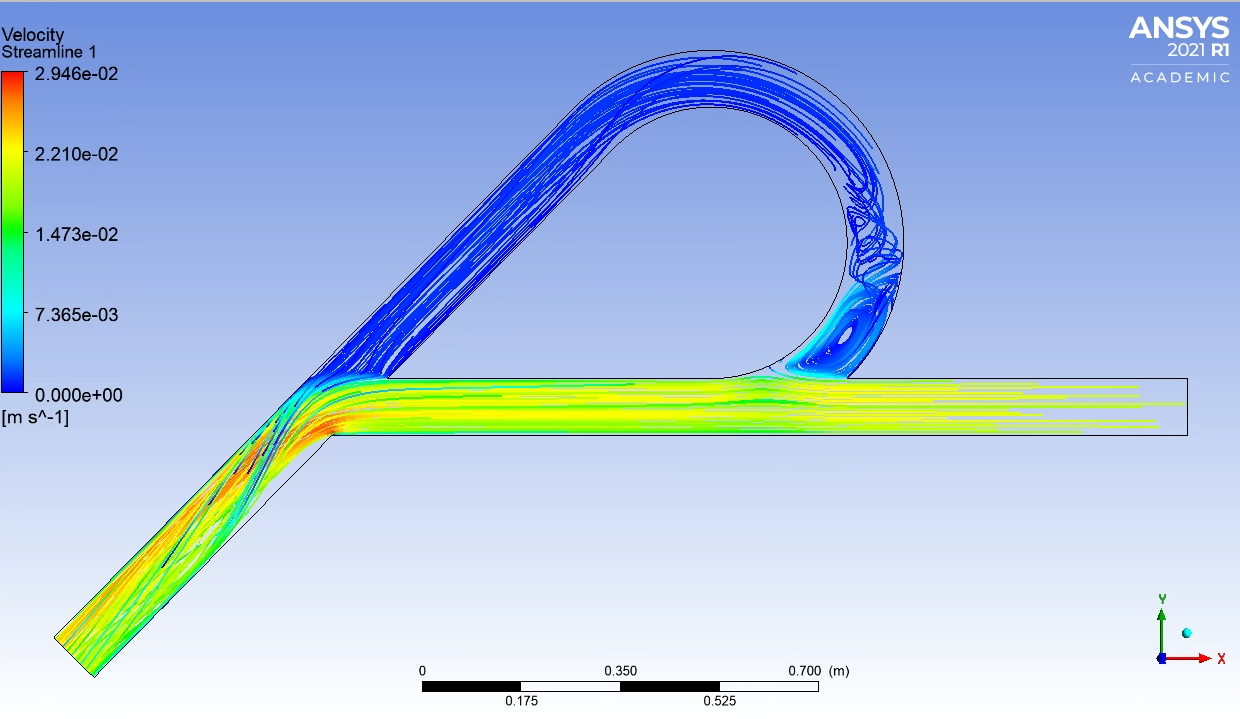
\includegraphics[width=.94\linewidth]{images/task3/epsilon_forward_streamline.png}
  \caption{$k-\epsilon$ Forward Flow Streamlines}
  \label{fig:x_d_norm}
\end{subfigure}%
~
\begin{subfigure}{.45\textwidth}
  \centering
  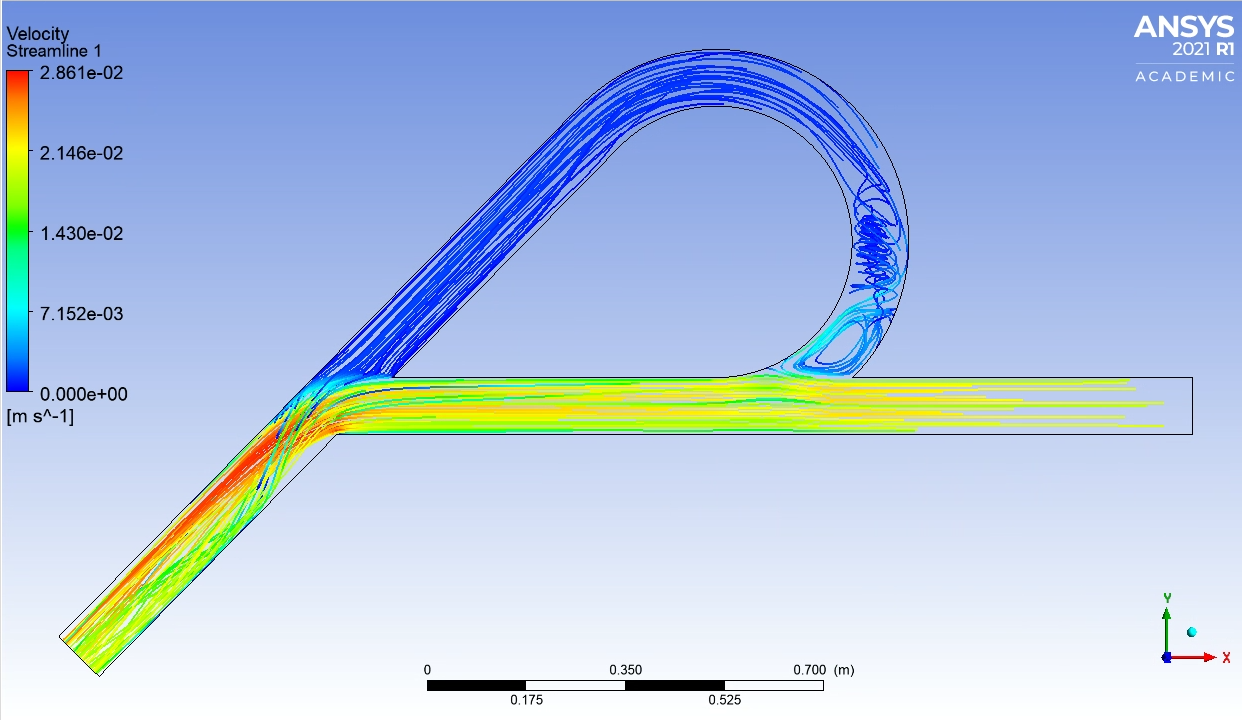
\includegraphics[width=.94\linewidth]{images/task3/omega_forward_streamline.png}
  \caption{$k-\omega$ Forward Flow Streamlines}
  \label{fig:x_d_norm_actual}
\end{subfigure}
~
\begin{subfigure}{.45\textwidth}
  \centering
  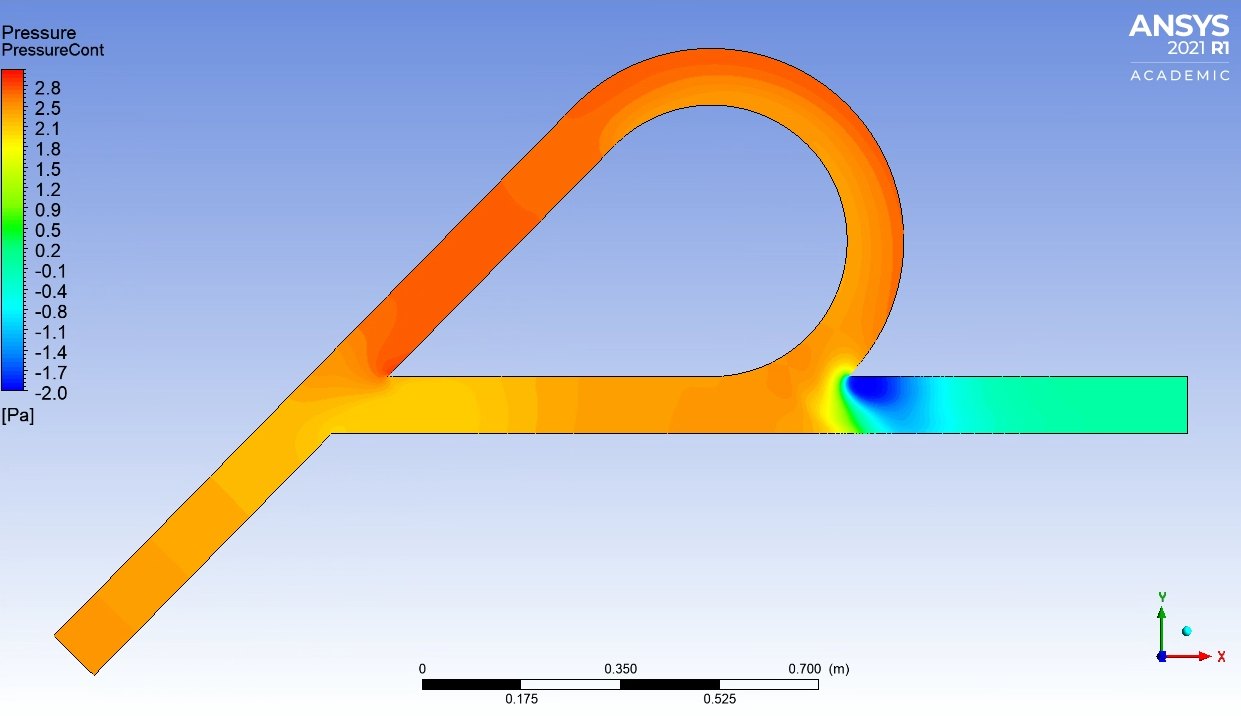
\includegraphics[width=.94\linewidth]{images/task3/epsilon_reverse_pressure.png}
  \caption{$k-\epsilon$ Backward Flow Pressure Contours}
  \label{fig:x_d_norm}
\end{subfigure}%
~
\begin{subfigure}{.45\textwidth}
  \centering
  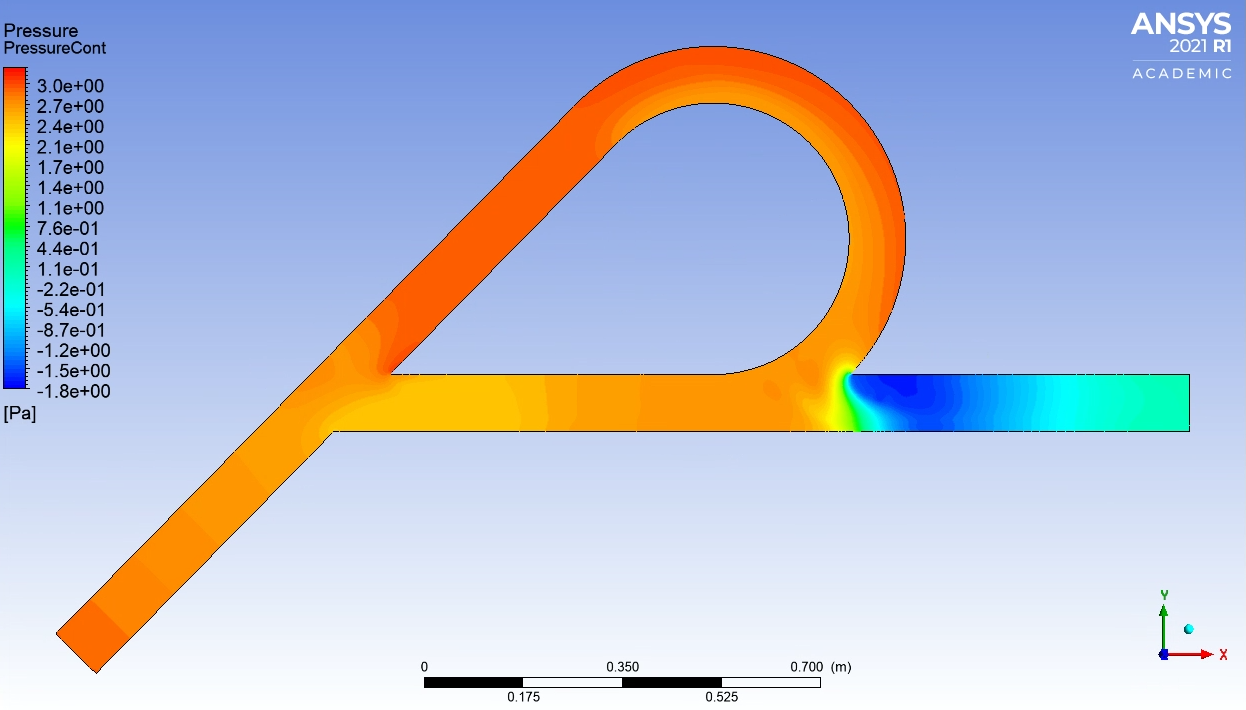
\includegraphics[width=.94\linewidth]{images/task3/omega_backward_pressure.png}
  \caption{$k-\omega$ Backward Flow Pressure Contours}
  \label{fig:x_d_norm_actual}
\end{subfigure}
~
\begin{subfigure}{.45\textwidth}
  \centering
  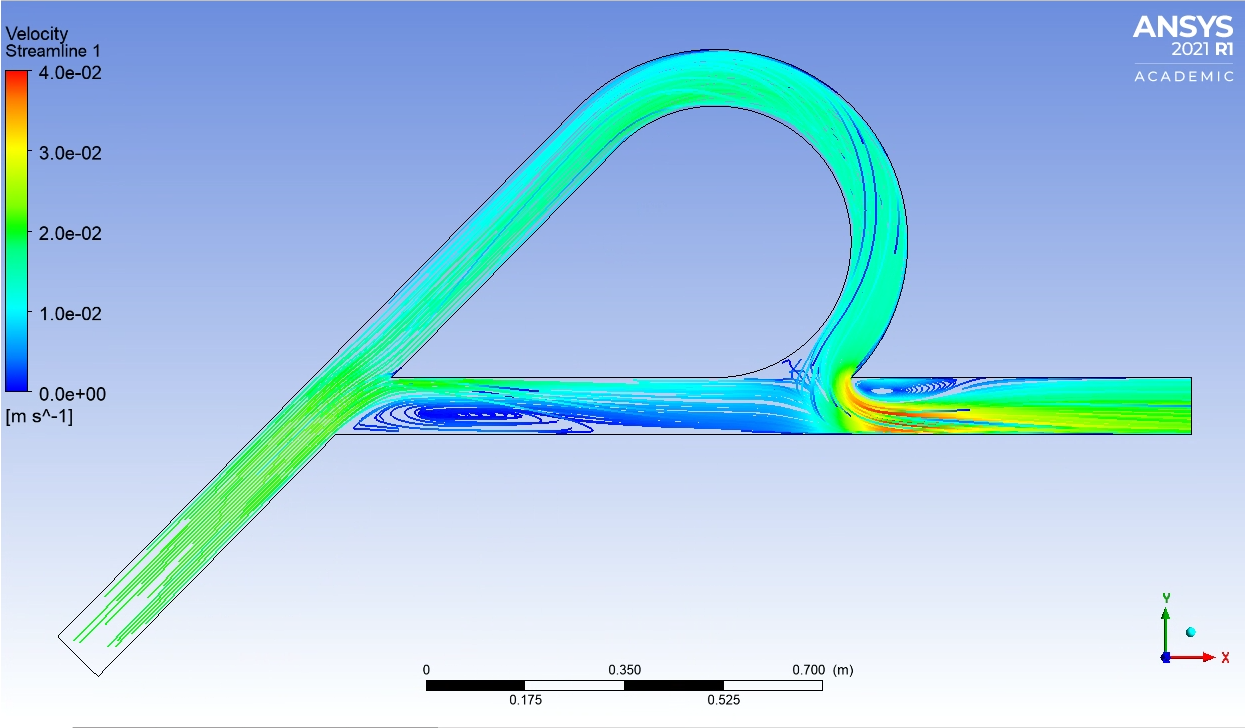
\includegraphics[width=.94\linewidth]{images/task3/epsilon_reverse_streamline.png}
  \caption{$k-\epsilon$ Backward Flow Streamlines}
  \label{fig:x_d_norm}
\end{subfigure}%
~
\begin{subfigure}{.45\textwidth}
  \centering
  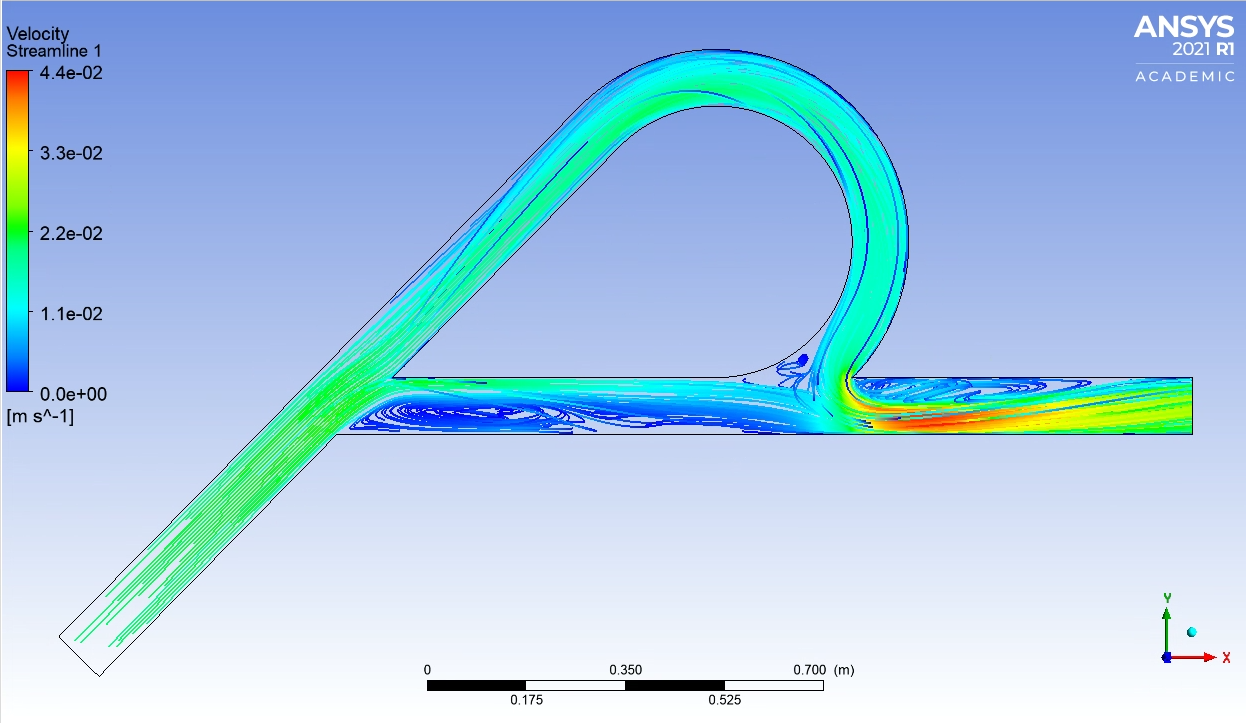
\includegraphics[width=.94\linewidth]{images/task3/omega_backward_streamline.png}
  \caption{$k-\omega$ Backward Flow Streamlines}
  \label{fig:x_d_norm_actual}
\end{subfigure}
~
\caption{Comparison of Turbulence Models}
\label{fig:omega_epsilon}
\end{figure}